\section{Durchführung}
\label{sec:Durchführung}

\subsection{Allgemein}

Bei dem Versuch sind vier Probestäbchen (zwei Messingstäbe mit unterschiedlichen 
Querschnittsflächen sowie jeweils ein Aluminiumstab und ein Edelstahlstab mit gleichen 
Querschnittsflächen) auf einer Platte befestigt. Wie der Abbildung \ref{fig:durchfuehrungbild1}
entnommen werden kann, werden die Stäbe an einer Seite mithilfe eines Peltierelements 
simultan erhitzt beziehungsweise abgekühlt. An jedem Stab befinden sich zwei Thermoelemente,
mit denen die Temperatur an dem Stab gemessen werden kann. Die Grundplatte ist zusätzlich mit 
dem 'XPlorer GLX' (Datenlogger) verbunden, welcher die aufgenommenen
Daten während der Messung anzeigen, aber auch abspeichern kann. Während der Messung soll die 
Wärmeisolierung über die Stäbe gelegt werden, damit die Abgabe von Wärme an die Umgebung so 
gering die möglich gehalten werden kann. 


\begin{figure}[H]
    \centering
    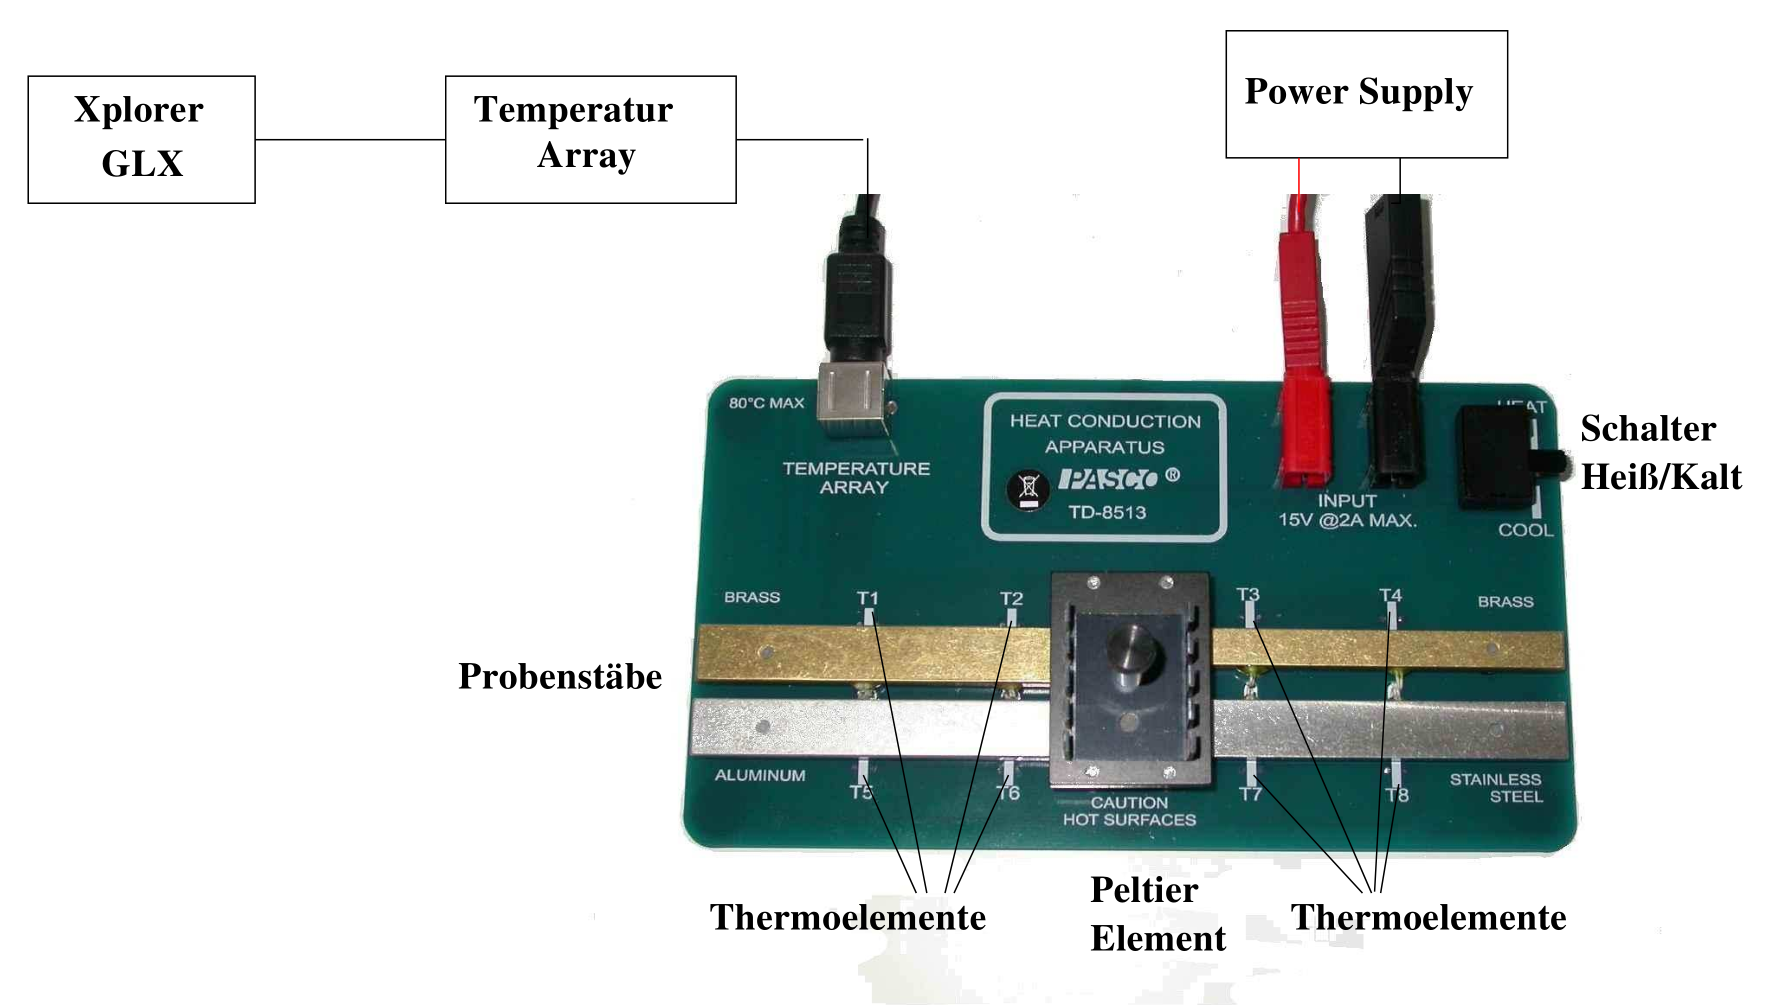
\includegraphics[width=13cm]{content/durchfuehrung1.png}
    \label{fig:durchfuehrungbild1}
    \caption{NAMENAMENAMENAME}
\end{figure}


\subsection{Statische Methode}

Zunächst soll der Abstand der Thermoelemente eines Stabes voneinander gemessen werden.
Die Abtastrate des Datenloggers soll auf $\Delta t_{GLX} = 5\, \si{\second}$ eingestellt werden.
Die mit der Grundplatte verbundene Spannungsquelle soll auf $U_P = 5\, \si{\volt}$ eingestellt 
werden. Wenn die Isolierung auf die Stäbe gelegt wurde, kann der Schalter an der Grundplatte auf
'Heat' umgelegt und die Messung gestartet werden. Die Messung soll beendet werden, wenn die 
Temperatur an Thermoelement $T_7$ ungefähr 45°C beträgt. Ist dieser Punkt erreicht, so sollen 
die Isolierungen abgenommen werden und der Schalter an der Grundplatte soll von 'Heat' auf
'Cool' umgelegt werden. Die aufgenommenen Daten, welche auf dem Datenlogger gespeichert wurden,
sollen grafisch ausgewertet werden. Erst wenn die Temperatur aller Thermoelemente unter 30°C 
liegt kann mit der zweiten Messung fortgefahren werden.



